\documentclass[convert={outfile=\jobname.png}]{standalone}
\usepackage{base}
\usepackage{draw}

\begin{document}

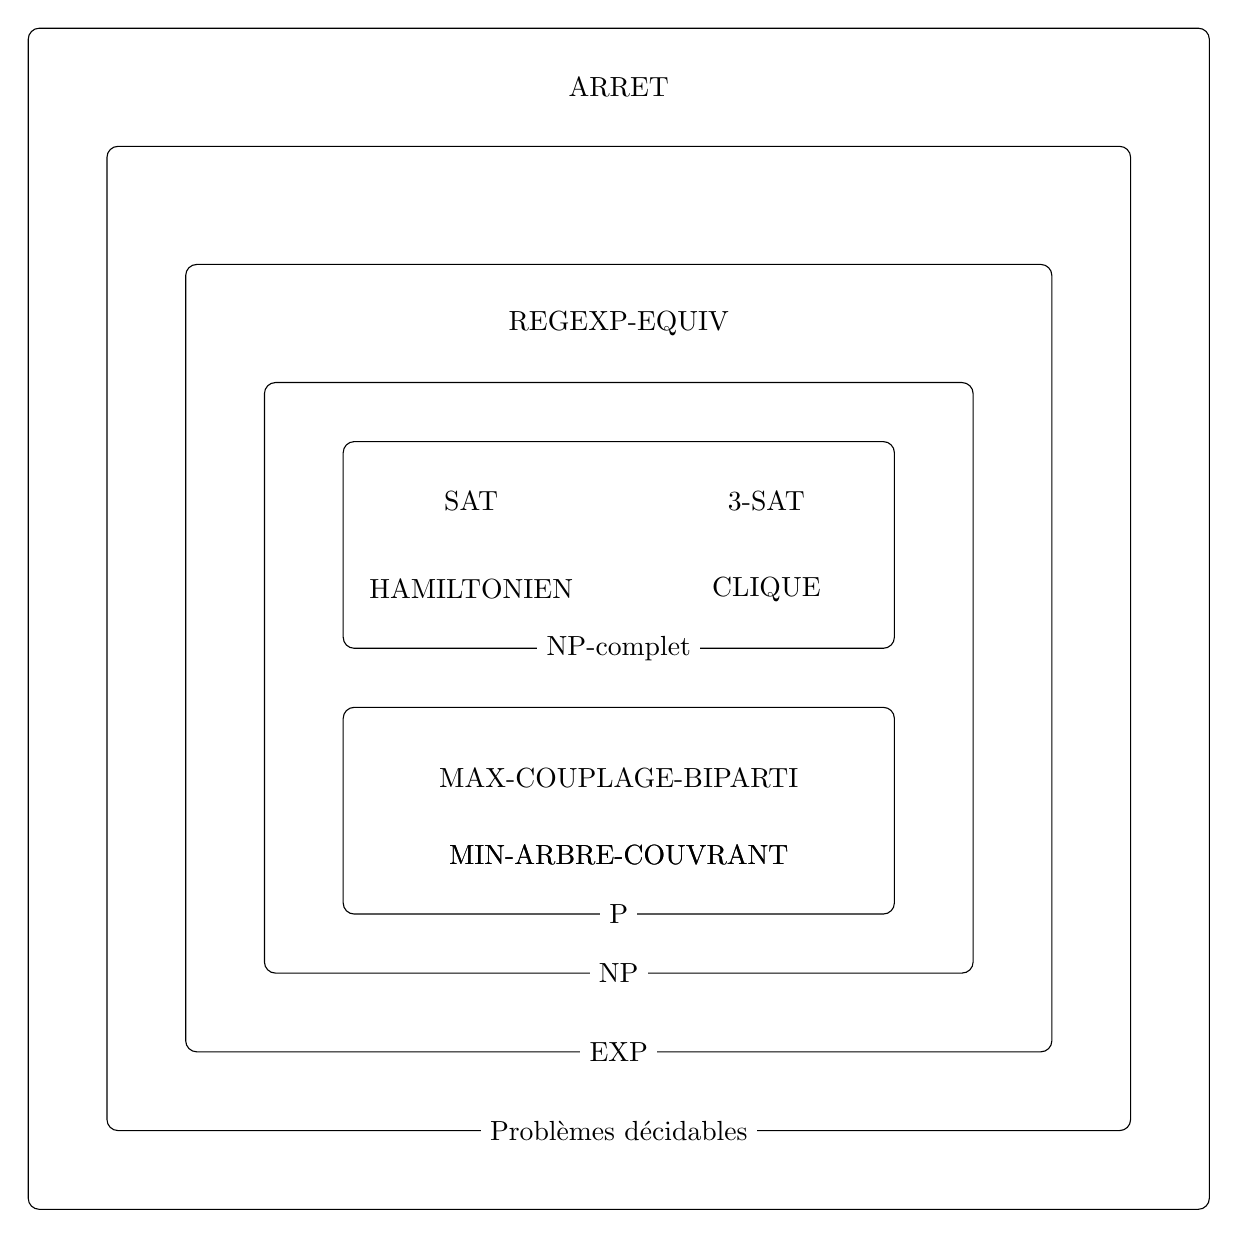
\begin{tikzpicture}
    \def\w{15}
    \def\h{15}
    \draw[rounded corners] (0, 0) rectangle (\w, \h);
    \node[fill=white] at (.5*\w, ) {Problèmes de décision};
    \node[] at (.5*\w, .95*\h) {ARRET};
    \draw[rounded corners] (1, 1) rectangle (\w - 1, .9*\h);
    \node[fill=white] at (.5*\w, 1) {Problèmes décidables};
    \draw[rounded corners] (2, 2) rectangle (\w - 2, .8*\h);
    \node[fill=white] at (.5*\w, 2) {EXP};
    \node[] at (.5*\w, .75*\h) {REGEXP-EQUIV};
    \draw[rounded corners] (3, 3) rectangle (\w - 3, .7*\h);
    \node[fill=white] at (.5*\w, 3) {NP};
    \draw[rounded corners] (4, 3.75) rectangle (\w - 4, .425*\h);
    \node[fill=white] at (.5*\w, 3.75) {P};
    \draw[rounded corners] (4, .65*\h) rectangle (\w - 4, .475*\h);
    \node[fill=white] at (.5*\w, .475*\h) {NP-complet};
    \node[] at (.5*\w, .365*\h) {MAX-COUPLAGE-BIPARTI};
    \node[] at (.5*\w, 4.5) {MIN-ARBRE-COUVRANT};
    \node[] at (.375*\w, .6*\h) {SAT};
    \node[] at (.625*\w, .6*\h) {3-SAT};
    \node[] at (.375*\w, .525*\h) {HAMILTONIEN};
    \node[] at (.625*\w, .525*\h) {CLIQUE};
    \node[] at (.5*\w, 4.5) {MIN-ARBRE-COUVRANT};
\end{tikzpicture}

\end{document}
